\chapter{Attention Mechanisms and Context Processing}

\section*{Why This Matters}

Attention mechanisms represent the architectural innovation enabling modern language models to process context effectively. Understanding attention—how it works, what computational costs it imposes, and how it scales—is essential for evaluating model capabilities, predicting performance characteristics, and assessing infrastructure requirements for context-intensive applications.

The attention mechanism's computational characteristics differ fundamentally from traditional neural network operations. While feed-forward layers scale linearly with input length, attention scales quadratically. This scaling behavior has direct implications for cost, latency, and feasible context lengths. A model processing 512 tokens requires 4× more attention computation than one processing 256 tokens, not 2×.

This chapter examines attention mechanisms from an engineering perspective, focusing on resource requirements, scaling behavior, and the trade-offs inherent in different attention configurations.

\section*{Key Questions This Chapter Answers}

By the end of this chapter, you'll be able to answer:

\begin{itemize}
    \item Why does doubling context length quadruple attention costs?
    \item When should you pay 4× more for efficient attention variants?
    \item What drives the practical 2K-8K token context limits you see in production?
    \item When does retrieval augmentation beat long-context models economically?
    \item How do you evaluate vendor claims about "advanced attention mechanisms"?
\end{itemize}

\section{Attention Mechanism Fundamentals}

\subsection{Selective Information Retrieval}

Attention mechanisms enable models to selectively focus on relevant information within input sequences. Rather than processing all input uniformly, attention computes relevance scores determining which parts of the input receive emphasis when processing each output position.

For language processing, this capability is essential. When processing "The company announced strong earnings, and its stock price rose 15\%," understanding "its" requires attending to "company" despite intervening words. Attention mechanisms implement this selective focus through learned relevance computations.

The mechanism operates through three components: queries (what we're looking for), keys (what information is available), and values (the actual information to retrieve). Each input position generates all three, enabling the model to determine which positions are relevant to which other positions.

\subsection{Query-Key-Value Architecture}

\textbf{The Library Search Analogy}

Imagine you're researching a topic in a library. Your Query (Q) is your search question—"What caused the 2008 financial crisis?" Keys (K) are index cards describing each book—"Banking regulation," "Mortgage markets," "Risk management." Values (V) are the actual books on the shelves.

The attention mechanism compares your Query against all Keys (which books are relevant?), computes relevance scores (banking regulation: 0.9, weather patterns: 0.01), and retrieves Values weighted by relevance (reads the relevant books, ignores irrelevant ones).

This three-part system exists because finding what's relevant (Q-K matching) is different from using what's relevant (V retrieval). You need index cards separate from the books themselves—otherwise you'd have to skim every book to know if it's useful.

\textbf{Why This Design?} Separating Q, K, V allows the model to learn both "how to search" and "what to retrieve" independently, making attention far more flexible than simple pattern matching.

The attention mechanism transforms input through three learned projections:

\textbf{Query Projection}: Converts each position's representation into a "search query" encoding what information that position needs.

\textbf{Key Projection}: Converts each position's representation into a "key" encoding what information that position contains.

\textbf{Value Projection}: Converts each position's representation into the actual information to be retrieved.

For BERT-base with 768-dimensional representations, each projection is a 768×768 matrix. Processing a 512-token sequence requires three matrix multiplications: input (512×768) times projection (768×768), yielding queries, keys, and values each sized 512×768.

The attention computation then determines relevance by comparing queries to keys. For each query position, the model computes similarity scores with all key positions, producing a 512×512 attention matrix. These scores determine how much each position attends to each other position.

\textbf{Why Three Separate Matrices?}

You might wonder: why not just use one matrix instead of Query, Key, Value? Consider the library analogy: Your question (Query) is different from the index system (Keys), and the index system is different from the actual books (Values). If you merged them, questions would need to match book content directly (no abstraction), the system couldn't learn "this type of question maps to these types of books," and flexibility would be lost.

The benefit of separate Q, K, V: The model learns how to ask (transform input into query representation), how to search (what makes things relevant—dot product of Q and K), and what to retrieve (the actual information—Values). This three-part separation is why attention is so powerful compared to simple pattern matching.

\subsection{Computational Characteristics}

The attention mechanism's computational cost has two primary components:

\textbf{Projection Operations}: Three matrix multiplications (Q, K, V) each requiring O(n·d²) operations, where n is sequence length and d is dimension. For BERT-base processing 512 tokens: 3 × 512 × 768² $\approx$ 900 million operations.

\textbf{Attention Computation}: Computing the 512×512 attention matrix and using it to weight values requires O(n²·d) operations. For BERT-base: 512² × 768 $\approx$ 200 million operations.

The critical observation: projection operations dominate for short sequences, but attention computation dominates for long sequences due to its quadratic scaling. At 512 tokens, projections require 4.5× more computation than attention. At 2048 tokens, attention requires 1.8× more computation than projections.

\subsection{Context Length Optimization Strategy}

This crossover behavior determines optimization priorities based on sequence length. For sequences under 512 tokens, attention optimization provides minimal return on investment since projection operations dominate computational cost. Resources are better spent on feed-forward acceleration and operator fusion, which address the actual bottlenecks.

For sequences between 512 and 2048 tokens, attention optimization becomes critical as attention computation represents 30-50\% of total work. Flash Attention 2.0, which has become standard practice by 2026, provides 3-5× speedup with zero quality loss—a mandatory optimization at this scale. Flash Attention 3 (released 2025) further improves memory efficiency by 8× and speeds up inference by an additional 20-30\%. Additional techniques like head pruning can provide another 10-20\% improvement for applications where the accuracy trade-off is acceptable.

For sequences exceeding 2048 tokens, attention computation consumes more than 60\% of total resources, fundamentally changing optimization priorities. At this scale, sparse or local attention variants become necessary, providing 4-16× computation reduction with typically less than 1\% quality loss. For inference workloads, Grouped-Query Attention (GQA) or Multi-Query Attention (MQA) reduce KV cache requirements by 4-8×, enabling larger batch sizes and higher throughput. These longer contexts may require architectural changes rather than simple optimizations.

The crossover point around 768 tokens determines when optimization focus must shift from feed-forward layers to attention mechanisms. Understanding this transition is essential for allocating engineering resources effectively.

\begin{figure}[htbp]
\centering
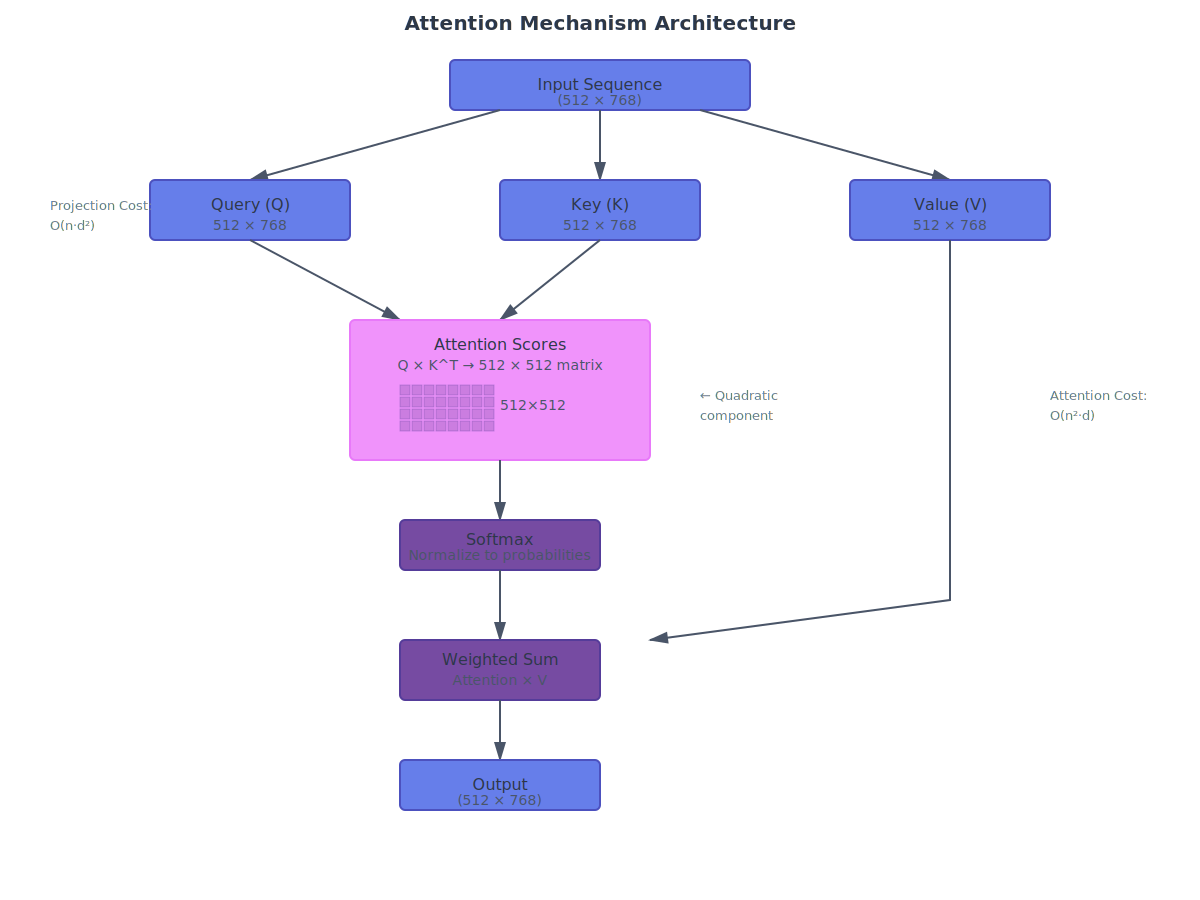
\includegraphics[width=0.95\textwidth]{chapters/diagrams/chapter03_attention_architecture_a1b2c3d4.pdf}
\caption{Attention mechanism architecture showing query-key-value projections and attention score computation. The quadratic attention matrix (n×n) drives memory and computational scaling for long sequences.}
\label{fig:attention_architecture}
\end{figure}


\section{Multi-Head Attention}

\subsection{Parallel Attention Mechanisms}

Multi-head attention employs multiple attention mechanisms in parallel, each learning different relevance patterns. BERT-base uses 12 attention heads per layer. Rather than one 768-dimensional attention mechanism, it implements 12 parallel 64-dimensional mechanisms.

The dimensional allocation: 768 dimensions divided across 12 heads yields 64 dimensions per head. Each head has its own Q, K, V projections (768×64 matrices) and produces 64-dimensional outputs. The 12 head outputs concatenate to reconstruct the full 768-dimensional representation.

This parallelization provides two benefits: diverse attention patterns (different heads learn different relevance criteria) and computational efficiency (smaller matrices enable better hardware utilization).

\subsection{Resource Implications}

Multi-head attention's resource requirements match single-head attention despite the parallelization. The total parameter count remains the same: whether implemented as one 768×768 projection or twelve 768×64 projections, the total is 768² parameters per projection type.

The computational cost similarly remains O(n·d²) for projections and O(n²·d) for attention computation. The multi-head structure reorganizes computation without changing total work.

The practical benefit: modern GPUs execute parallel operations efficiently. Twelve 64-dimensional attention computations often execute faster than one 768-dimensional computation due to better cache utilization and parallelism exploitation.

\subsection{Head Specialization}

Empirical analysis reveals that attention heads learn specialized roles. Some heads focus on syntactic relationships (subject-verb agreement), others on semantic relationships (coreference resolution), and others on positional patterns (attending to adjacent tokens).

This specialization has optimization implications. Research demonstrates that many heads contribute minimally to model performance—pruning 20-30\% of heads typically degrades accuracy by less than 1\%. For production deployments, head pruning represents a viable optimization strategy, reducing computation by 20-30\% with minimal quality impact.

\begin{figure}[htbp]
\centering
\includegraphics[width=0.9\textwidth]{chapters/diagrams/chapter03_multihead_attention_e5f6g7h8.pdf}
\caption{Multi-head attention parallel computation structure. Twelve 64-dimensional heads process independently, then concatenate. This structure enables efficient GPU utilization while learning diverse attention patterns.}
\label{fig:multihead_attention}
\end{figure}


\section{Context Length and Scaling Behavior}

\subsection{Quadratic Scaling Characteristics}

Attention's quadratic scaling with sequence length represents its most significant computational characteristic. Doubling context length quadruples attention computation and memory requirements.

For BERT-base:
\begin{itemize}
    \item 128 tokens: 128² = 16,384 attention scores per head
    \item 512 tokens: 512² = 262,144 attention scores per head (16× increase)
    \item 2048 tokens: 2048² = 4,194,304 attention scores per head (256× increase)
\end{itemize}

With 12 heads per layer and 12 layers, BERT-base computing 2048-token attention requires storing and computing approximately 600 million attention scores. At 4 bytes per score, this represents 2.4 GB of memory just for attention matrices—before considering activations, parameters, or gradients.

\subsection{Memory Bottlenecks}

For long-context applications, attention memory often becomes the limiting constraint before computational capacity. The attention matrix grows quadratically while other components grow linearly, causing attention to dominate memory consumption at sufficient length.

Memory allocation for 2048-token BERT-base processing reveals this pattern clearly. Attention matrices consume approximately 2.4 GB, representing 60\% of total memory. Other activations require approximately 1.2 GB (30\% of total), while parameters account for only 0.4 GB (10\% of total). This distribution explains why context length extensions require disproportionate memory increases.

Doubling context from 512 to 1024 tokens increases total memory requirements by approximately 3×, not 2×, due to attention's quadratic scaling. The attention matrix grows by 4× (from 512² to 1024²), while other components only double. This non-linear relationship makes memory planning for long-context applications particularly challenging.

\subsection{Practical Context Length Limits}

The quadratic scaling imposes practical limits on context length for standard attention mechanisms. On typical GPU hardware, these constraints manifest as hard memory limits that determine maximum feasible sequence lengths.

On an A100 GPU with 40 GB memory, BERT-base can process approximately 4096 tokens maximum. BERT-large, with its larger dimensional parameters, reaches its limit around 2048 tokens. At GPT-3 scale, the maximum drops to approximately 512 tokens due to the model's substantially larger parameter count and activation requirements.

These limits assume inference only. Training requires additional memory for gradients and optimizer states, reducing feasible context lengths by 2-3×. A model that can process 4096 tokens during inference might be limited to 1536 tokens during training on the same hardware.

For applications requiring longer context—document analysis, long-form generation, comprehensive code review—these constraints necessitate either architectural modifications through efficient attention variants or infrastructure investments in larger memory capacity or distributed processing across multiple GPUs.

\begin{figure}[htbp]
\centering
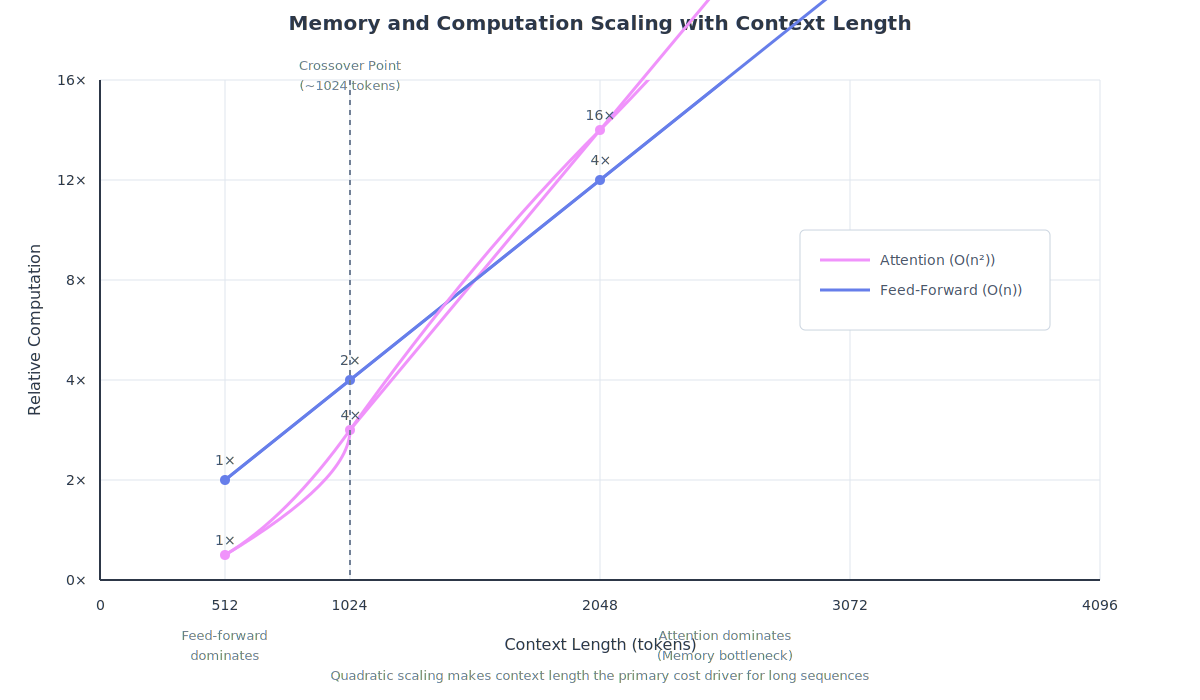
\includegraphics[width=0.9\textwidth]{chapters/diagrams/chapter03_context_scaling_i9j0k1l2.pdf}
\caption{Memory and computation scaling with context length. Attention (quadratic) dominates at longer contexts while feed-forward operations (linear) remain constant per token. The crossover point determines when context length becomes the primary cost driver.}
\label{fig:context_scaling}
\end{figure}


\section{Attention Patterns and Interpretability}

\subsection{Learned Attention Distributions}

Attention mechanisms learn which positions to emphasize through training. The resulting attention patterns provide insight into model behavior and can inform optimization decisions.

Trained models exhibit several common attention patterns. Local attention appears frequently, with many heads attending primarily to nearby tokens within approximately ±5 positions. This pattern suggests that local context often suffices for many language understanding tasks, motivating efficient attention variants that restrict attention to local windows rather than computing full quadratic attention.

Positional attention patterns emerge in some heads, which attend to specific relative positions such as the previous token or next token. These patterns are highly predictable and could potentially be hardcoded rather than learned, representing an optimization opportunity for specialized applications.

Semantic attention represents the model's long-range reasoning capability. Certain heads learn semantic relationships, attending to syntactically or semantically related tokens regardless of distance. These heads enable the model to resolve references, understand dependencies, and maintain coherence across long spans of text.

\subsection{Optimization Implications}

Understanding attention patterns enables targeted optimization strategies that trade some model expressiveness for substantial efficiency gains. The appropriate trade-off depends on application requirements and performance constraints.

Sparse attention mechanisms can skip low-weight computations when most attention weights are near-zero, as empirical analysis often reveals. This approach reduces computational work by 50-80\% with minimal accuracy impact, since the skipped computations contribute little to the final output.

Local attention windows restrict attention to fixed ranges, such as ±256 tokens, when attention is predominantly local. This restriction reduces complexity from O(n²) to O(n), enabling much longer contexts. For applications where most relevant information appears within local windows, this trade-off provides dramatic efficiency gains with acceptable accuracy.

Head pruning removes heads with minimal impact on downstream performance, reducing computation proportionally. Analysis of trained models often reveals that 20-30\% of attention heads contribute minimally to final performance, making them candidates for removal in production deployments where efficiency matters more than marginal accuracy improvements.


\section{Attention in Model Architecture}

\subsection{Attention Layers in Transformers}

Transformer architectures interleave attention layers with feed-forward layers. BERT-base's 12 layers each contain:
\begin{itemize}
    \item Multi-head attention sublayer (21M parameters, 40\% of layer computation)
    \item Feed-forward sublayer (4.7M parameters per layer, 60\% of layer computation)
\end{itemize}

Despite attention's conceptual importance, feed-forward layers consume more computation for typical sequence lengths ($\leq$512 tokens). At longer sequences, attention's quadratic scaling causes it to dominate.

The crossover point for BERT-base occurs around 1024 tokens. Below this length, feed-forward computation dominates; above it, attention dominates. This crossover point varies by model architecture and dimensional choices.

\subsection{Attention Versus Feed-Forward Trade-offs}

Model designers face trade-offs in allocating computational budget between attention and feed-forward components:

\textbf{More Attention Capacity}: Increasing attention heads or dimensions improves long-range reasoning but increases quadratic scaling costs.

\textbf{More Feed-Forward Capacity}: Increasing feed-forward dimensions improves per-token processing but doesn't enhance cross-token reasoning.

BERT-base allocates 52\% of parameters to feed-forward networks, 32\% to attention, and 16\% to embeddings. This distribution reflects empirical optimization across diverse tasks. Alternative allocations may be optimal for specific use cases (e.g., more attention for long-context tasks, more feed-forward for token-level tasks).


\section{Cost Analysis and Forecasting}

\subsection{Attention Cost Estimation}

Attention costs can be estimated using:

\begin{center}
\fbox{\parbox{0.8\textwidth}{
\centering
Attention Cost = Layers × Heads × (Projection Cost + Attention Matrix Cost)\\[0.5em]
Projection Cost = 3 × n × d²\\
Attention Matrix Cost = n² × d
}}
\end{center}

For BERT-base processing 512 tokens:
\begin{itemize}
    \item Projection: 12 layers × 12 heads × 3 × 512 × 64² $\approx$ 900M operations
    \item Attention: 12 layers × 12 heads × 512² × 64 $\approx$ 240M operations
    \item Total: $\sim$1.1B operations per forward pass
\end{itemize}

At 312 TFLOPS (A100 GPU) with 40\% efficiency: approximately 9 microseconds per forward pass for attention computation alone.

\subsection{Context Length Impact on Costs}

Context length directly impacts both latency and throughput:

\textbf{Latency}: Quadratic scaling means 4× context requires 4× more attention computation, increasing latency proportionally (assuming compute-bound).

\textbf{Throughput}: Longer contexts reduce batch sizes due to memory constraints, further reducing throughput. A 4× context increase might reduce throughput by 8-10× due to combined effects.

\textbf{Cost}: For inference-heavy applications, context length is a primary cost driver. Reducing average context length by 2× can reduce infrastructure costs by 3-4×.

\begin{tcolorbox}[colback=orange!5!white,colframe=orange!75!black,title=\textbf{MENTAL MODEL: Context Length Economic Threshold}]

\textbf{Principle:} Attention costs scale quadratically (O(n²)). Doubling context length quadruples attention cost, not doubles it.

\textbf{Economic Thresholds:}
\begin{itemize}
    \item Less than 512 tokens: Attention is cheap (less than 20\% of total cost)
    \item 512-2K tokens: Attention becomes significant (20-50\% of cost)
    \item 2K-8K tokens: Attention dominates (50-70\% of cost)
    \item Greater than 8K tokens: Consider alternatives (RAG, chunking, sparse attention)
\end{itemize}

\textbf{Decision Framework:}
\begin{enumerate}
    \item Calculate actual average context length needed (not worst-case)
    \item If greater than 4K tokens, evaluate RAG versus long-context
    \item RAG cost: (embedding + retrieval + generation with 4K context)
    \item Long-context cost: (generation with full context)
    \item Choose RAG if cost ratio exceeds 4× and quality gap is less than 5\%
\end{enumerate}

\textbf{Example:} Legal document analysis. Full contract: 50K tokens. Long-context model: (50/4)² equals 156× more expensive attention than 4K baseline. RAG approach: Chunk into 4K segments, retrieve top 3 relevant chunks, generate answer. Cost: approximately 10× cheaper with 2-3\% quality reduction.

\textbf{Red Flag:} "We need maximum context length available"—this often indicates lack of cost analysis. Question whether full context is necessary or retrieval would suffice.

\end{tcolorbox}

\subsection{Optimization ROI}

Attention optimization provides substantial returns for long-context or high-volume applications:

\textbf{Sparse Attention} (50-80\% computation reduction):
\begin{itemize}
    \item Implementation cost: 2-4 weeks engineering
    \item Accuracy impact: typically <1\%
    \item Cost savings: 50-80\% of attention computation (20-40\% of total)
\end{itemize}

\textbf{Head Pruning} (20-30\% computation reduction):
\begin{itemize}
    \item Implementation cost: 1-2 weeks analysis and validation
    \item Accuracy impact: typically <1\%
    \item Cost savings: 20-30\% of attention computation (8-15\% of total)
\end{itemize}

For systems processing millions of requests daily, these optimizations can reduce annual infrastructure costs by hundreds of thousands of dollars.


\section{Evaluation Framework}

\subsection{Attention Configuration Assessment}

When evaluating attention-related proposals, consider:

\textbf{Context Length Requirements}:
\begin{itemize}
    \item What context length is specified, and what is the justification?
    \item What percentage of inputs actually require the maximum context length?
    \item Have shorter context alternatives been evaluated?
    \item What is the memory and computational cost at the proposed context length?
\end{itemize}

\textbf{Attention Architecture}:
\begin{itemize}
    \item How many attention heads are proposed? What is the empirical justification?
    \item What is the dimensional allocation per head?
    \item Have efficient attention variants been considered (sparse, local, etc.)?
    \item What is the expected attention pattern (local, global, semantic)?
\end{itemize}

\textbf{Optimization Strategy}:
\begin{itemize}
    \item What is the plan for handling variable-length inputs efficiently?
    \item Have attention optimizations (pruning, sparsity) been evaluated?
    \item What is the memory budget, and how does attention fit within it?
    \item What is the latency target, and how does attention computation impact it?
\end{itemize}

\subsection{Common Assessment Pitfalls}

\textbf{Overspecifying Context Length}: Many applications specify maximum context length based on worst-case scenarios rather than typical usage. If 95\% of inputs use $\leq$512 tokens, optimizing for 2048-token maximum wastes resources.

\begin{tcolorbox}[colback=red!5!white,colframe=red!75!black,title=\textbf{COMMON MISTAKE: Optimizing for Maximum Context Length}]

\textbf{What Happened}:
\begin{itemize}
    \item Client requirement: "We need to handle documents up to 50,000 tokens"
    \item Team optimizes for 50k context: implements sparse attention, 6 weeks of work
    \item Actual usage distribution: 95\% of documents are <4,000 tokens
    \item 50k+ documents: <0.1\% of traffic
\end{itemize}

\textbf{Cost of mistake}: \$150,000 in engineering costs + 6 weeks delay + ongoing 3× higher infrastructure costs for edge cases

\textbf{What should have happened}:
\begin{enumerate}
    \item Analyze actual document distribution first (1 day)
    \item Optimize for the 95th percentile (4k tokens)
    \item Handle 50k+ edge cases separately (chunking, summarization, or dedicated pipeline)
    \item Total cost: \$10,000 + 1 week
\end{enumerate}

\textbf{Lesson}: Base architectural requirements on actual usage distribution, not worst-case scenarios. Measure first, optimize second.

\end{tcolorbox}

\textbf{Ignoring Quadratic Scaling}: Linear thinking about context length leads to underestimated costs. Doubling context doesn't double costs—it typically triples or quadruples them due to attention's quadratic scaling.

\textbf{Uniform Attention Assumptions}: Assuming all positions need to attend to all other positions ignores empirical attention patterns. Most applications can benefit from sparse or local attention with minimal accuracy impact.

\textbf{Neglecting Batch Size Impact}: Longer contexts reduce feasible batch sizes, compounding throughput impacts. A proposal for 4× longer context may reduce throughput by 8-10×, not 4×.

\section{Where You'll See This in Practice}

Attention mechanisms are the architectural innovation that enabled modern LLMs. Understanding their cost structure (quadratic scaling) and optimization opportunities shapes decisions across all domain applications. The following examples show how Chapter 3's concepts directly inform real-world decisions you'll face when evaluating AI proposals.

\subsection{Legal Discovery (Chapter 13.5)}

E-discovery systems processing thousands of documents face context length explosion: Depositions and contracts span 20-100 pages (50K-250K tokens). Quadratic cost impact (Section 3.3.1): 100-page document costs 25× more attention compute than 20-page document. Practical solution: Chunking plus retrieval (Chapter 5.7 RAG) versus long-context models.

\textbf{Real scenario}: Law firm evaluating document review platform. Vendor A: "We use 128K context windows to analyze full contracts." Vendor B: "We chunk documents and use RAG with 4K context." Cost analysis (using Section 3.6): Vendor A: 128K context equals (128/4)² equals 1024× more expensive attention. Vendor B: 4K context plus retrieval overhead approximately 10× cheaper. Quality: Vendor A slightly better, Vendor B "good enough" (95\% versus 97\%). Decision: Vendor B—10× cost savings justifies 2\% quality gap.

\textbf{Decision point}: When vendors tout "long context windows," ask: What's the per-document cost? Would chunking plus retrieval be more economical? Section 3.6.2 provides the calculation framework.

\subsection{Healthcare Clinical Notes (Chapter 12.2)}

Clinical NLP systems processing patient records involve multi-head attention (Section 3.2): Different heads learn symptom patterns, medication interactions, timeline relationships. Context length constraints (Section 3.3.3): Patient histories span years but models limited to 4K-8K tokens. Head specialization (Section 3.2.3): Medical terms, temporal relationships, entity recognition each use different attention heads.

\textbf{Real scenario}: Hospital implements clinical decision support. Challenge: Patient has 10-year history (500K tokens), model supports 8K tokens. Naive approach: Truncate to most recent 8K tokens, misses critical historical events. Attention-aware approach: Use retrieval to select relevant historical events based on current symptoms (Section 3.4). Result: 8K token context with curated history outperforms 32K token chronological history.

\textbf{Decision point}: Section 3.3.3's practical limits help you evaluate whether "we need longer context" or "we need smarter retrieval."

\subsection{Financial Time-Series Analysis (Chapter 14.1)}

Algorithmic trading models face temporal attention patterns (Section 3.4.1): Recent price movements weighted more heavily than historical. Multi-head specialization (Section 3.2.3): Different heads learn intraday patterns, weekly trends, earnings cycles. Latency requirements: Flash Attention (Section 3.6.3) becomes critical for microsecond trading decisions.

\textbf{Real scenario}: Hedge fund evaluating temporal fusion transformer (TFT) versus ARIMA. TFT (attention-based): Learns complex interactions, requires GPU, 10ms latency. ARIMA (statistical): Fast (1ms), interpretable, but can't capture non-linear patterns. Performance: TFT improves Sharpe ratio from 1.5 to 1.8 (20\% improvement). Decision: Deploy TFT for signals, ARIMA for risk checks (hybrid approach).

\textbf{Decision point}: Section 3.2.3's head specialization helps you understand when attention-based models justify their computational cost over simpler alternatives.

\subsection{Code Completion (Chapter 11.2)}

GitHub Copilot-style systems involve context optimization (Section 3.1.4): How much code history to include? Attention cost at scale: Millions of autocomplete requests daily. Multi-head patterns (Section 3.2.1): Different heads learn syntax, semantics, cross-file references.

\textbf{Real scenario}: Company building internal code completion tool. Challenge: Include full file (2K tokens) versus recent function (512 tokens)? Cost analysis (Section 3.3.1): 2K context costs (2000/512)² equals 15× more. Quality analysis: Full file gives 2-3\% better completions. Volume: 10M requests/day equals \$30K/day (full context) versus \$2K/day (function only). Decision: Function-only context—\$10M/year savings not justified by 2-3\% quality gain.

\textbf{Decision point}: Section 3.6.1's cost estimation framework helps you quantify the quality-cost trade-off in per-request economics.

\subsection{Semantic Search (Chapter 10.2)}

Enterprise search with RAG involves attention efficiency: Embedding models (BERT) versus generation models (GPT). Bi-directional attention (Section 3.1.2): BERT's advantage for encoding queries and documents. Cost structure: Embeddings cheap (\$0.0001/query), generation expensive (\$0.01/query).

\textbf{Real scenario}: Company deploying enterprise knowledge base search. Approach 1: Pure GPT-4—powerful but \$0.03 per query. Approach 2: BERT embeddings (\$0.0001) plus GPT-3.5 generation (\$0.002) equals \$0.0021 per query. Volume: 100K queries/month. Cost: \$3,000/month (Approach 1) versus \$210/month (Approach 2)—14× cheaper. Quality: Approach 2 slightly worse (90\% versus 94\% relevance) but acceptable.

\textbf{Decision point}: Understanding attention mechanisms (this chapter) helps you architect hybrid systems that use cheap attention (embeddings) for retrieval and expensive attention (LLMs) only for generation.

\subsection{Key Patterns: When Attention Costs Dominate}

\textbf{Attention is your bottleneck when}: Long documents (greater than 4K tokens)—costs scale quadratically (Section 3.3.1). High request volume (greater than 1M/day)—attention compute dominates total cost. Real-time requirements—efficient attention variants become critical.

\textbf{Attention costs are negligible when}: Short contexts (less than 512 tokens)—feed-forward layers dominate. Batch processing—amortize attention overhead across many examples. Low request volumes—fixed infrastructure costs dominate.

Use Section 3.6's cost analysis frameworks to determine which category your use case falls into—this determines whether attention optimization is critical or irrelevant to your budget.

\subsection{Decision Checklist: Evaluating Attention-Related Proposals}

When your team proposes attention-based architectures, verify: Context length specified and justified? (Section 3.3.3). Cost calculated for quadratic scaling with context length? (Section 3.3.1). Compared long-context versus retrieval augmentation? (Section 3.1.4). Considered efficient attention variants (Flash, sparse)? (Section 3.4.2, 6.3). Estimated per-request cost at production volume? (Section 3.6).

\textbf{Red flags}: "We need the longest context window available" (May not justify 4-16× cost increase). No mention of retrieval alternatives (Missing 10× cheaper option). Linear cost scaling assumed for context length (Ignoring quadratic reality). "Attention is cheap" with greater than 4K context (Misunderstanding of Section 3.3.1).

Chapter 3's frameworks will save you from approving architectures that work in development but become prohibitively expensive at production scale.

\section{Key Insights}

\textbf{Quadratic Scaling}: Attention computation and memory scale quadratically with sequence length. Doubling context length quadruples attention costs, making context length a primary cost driver for long-sequence applications.

\textbf{Memory Dominance}: For sequences beyond 1024 tokens, attention matrices typically consume 50-70\% of total memory. Memory constraints often limit context length before computational constraints.

\textbf{Multi-Head Benefits}: Multi-head attention provides diverse attention patterns without increasing total computation. The parallel structure also enables better hardware utilization on modern GPUs.

\textbf{Optimization Opportunities}: Most models can reduce attention computation by 50-80\% through sparse attention, head pruning, or local attention windows with minimal accuracy impact (<1\% typically).

\textbf{Context Length Trade-offs}: Maximum context length should be determined by typical usage patterns, not worst-case scenarios. Overspecifying context length wastes substantial resources due to quadratic scaling.

\textbf{Crossover Behavior}: For BERT-scale models, attention dominates computation above $\sim$1024 tokens; feed-forward layers dominate below. This crossover point informs optimization priorities.

The next chapter examines training transformers—how attention mechanisms are optimized during training, what additional memory requirements emerge, and how distributed training strategies address scale challenges.
